\capitulo{3}{Conceptos teóricos}

\section{Inteligencia artificial}

Un concepto tan amplio como lo es la inteligencia artificial se puede definir de múltiples formas, a continuación se citan algunas:

\begin{enumerate}
    \item <<La habilidad, como sistema, de interpretar correctamente datos externos, aprender de estos datos, y usar lo aprendido para lograr objetivos y tareas concretas a través de una adaptación flexible>> \cite{kaplan_haenlein_2019}.
    \item <<... la habilidad de un sistema de actuar adecuadamente en un ecosistema incierto en el que la acción apropiada es la que aumenta la probabilidad de alcanzar el objetivo, siendo el objetivo completar una serie de logros menores que ayuden a alcanzar el objetivo final>> \cite{albus_1991}.
    \item <<Estudio de del diseño de agentes inteligentes>> \cite{poole_mackworth_goebel_1998}.
\end{enumerate}

\subsection{Historia de la inteligencia artificial}
Durante la segunda guerra mundial, el aclamado científico Alan Turing descifró el <<Código Enigma>> usado por las fuerzas alemanas para mandar mensajes de forma segura. Alan Turing y Enigma conforman los pilares de la inteligencia artificial y el \english{machine learning}.

En 1956, el científico John McCarthhy\footnote{\url{https://es.wikipedia.org/wiki/John\_McCarthy}}, usó el término inteligencia artificial por primera vez en la Conferencia Dartmouth\footnote{\url{https://es.wikipedia.org/wiki/Conferencia\_de\_Dartmouth}}, dando lugar a la creación de varios centros de investigación en Estados Unidos con el propósito del estudio del potencial de la inteligencia artificial. Los investigadores Allen Newell\footnote{\url{https://es.wikipedia.org/wiki/Allen\_Newell}} y Herbert Simon\footnote{\url{https://es.wikipedia.org/wiki/Herbert\_Alexander\_Simon}}  fueron clave para impulsar inteligencia artificial como un nuevo campo en la Informática que podría cambiar el mundo.

A partir de los años 60, el principal enfoque de los investigadores se centró en desarrollar algoritmos para resolver problemas y teoremas matemáticos. Este proceso dio lugar a los primeros conceptos sobre \english{machine vision learning}\footnote{\url{https://es.wikipedia.org/wiki/Vision\_artificial}} y inteligencia artificial aplicada a la robótica.

Tras un largo periodo sin avances notables debido a una escasez de financiaciones para el desarrollo de la inteligencia artificial, a finales de los años 90, el desarrollo resurge gracias a grandes corporaciones interesadas en usar este campo para lograr unas ventajas y beneficios nunca vistos, Es así como en 1997 la máquina Deep Blue\footnote{\url{https://es.wikipedia.org/wiki/Deep_Blue_(computadora)}} de IBM se convirtió en la primera computadora capaz de derrotar a un campeón mundial de ajedrez como lo fue Garry Kasparov.

En los últimos 15 años, las principales empresas mundiales han utilizado la inteligencia artificial como una herramienta más a la hora de crecer y convertirse en el sector más importante del mundo, gracias a campos como la visión artificial, minería de datos o el procesamiento de lenguajes naturales \cite{aihistory}.

\subsection{Machine Learning (Aprendizaje automático)}
El \english{Machine Learning} se considera un campo de las ciencias de computación y a su vez una rama de la inteligencia artificial. Tiene como objetivo principal el desarrollo de técnicas y la búsqueda de algoritmos y heurísticas que permitan que las computadoras aprendan por si mismas a través de la experiencia.

Las aplicaciones que conforman este campo son muy variadas, desde su uso en diagnósticos médicos, análisis de patrones, reconocimiento de lenguajes naturales hablados y escritos, a juegos o robótica \cite{wiki:apredizaje_automatico}.

A su vez los diferentes algoritmos de aprendizaje automático se pueden agrupar por tipos según la salida de los mismos.
Encontramos así:

\begin{description}
    \item[Aprendizaje supervisado] Produce una función que establece una correspondencia entre las entradas y salidas deseadas. Un posible uso de estos algoritmos podría ser un problema de clasificación en el que hay que etiquetar una serie de valores usando una entre varias categorías. En este tipo de aprendizaje, la base del conocimiento estaría formada por ejemplos de etiquetados anteriores.
    
    \newpage
    
    \item[Aprendizaje no supervisado] En este caso el proceso se lleva a cabo por un conjunto de datos únicamente formado por entradas al sistema que no contienen información sobre las categorías de cada ejemplo. El sistema debe reconocer los patrones de forma autónoma para encontrar grupos de elementos comunes y asignar las nuevas entradas a dichos grupos.
    \item[Aprendizaje semi-supervisado] Estos algoritmos combinan los dos anteriores para clasificar teniendo en cuenta los datos clasificados y los no clasificados.
    \item[Aprendizaje por refuerzo] En este tipo de algoritmos, el sistema aprende observando lo que le rodea, es decir, su información de entrada se basa en la retroalimentación que obtiene como respuesta a sus acciones. Se podría decir que aprende a base de prueba-error.
    \item[Transducción] Un algoritmo similar al aprendizaje supervisado tratado anteriormente. La principal diferencia sería que no construye de forma explícita una función. Un posible ejemplo de este tipo de algoritmos sería el $k$ de vecinos mas cercanos\footnote{\url{https://es.wikipedia.org/wiki/K\_vecinos\_mas\_proximos}}.
    \item[Aprendizaje multi-tarea] Los métodos incluidos en esta categoría se basan en la utilización de el conocimiento aprendido previamente para enfrentarse a problemas similares a los ya vistos.
\end{description}

\section{Redes neuronales}
Una Red Neuronal Artificial (RNA) se basa en un modelo inspirado en el comportamiento de las neuronas y como se organizan para crear una estructura en el cerebro.

El cerebro se puede llegar a ver como un sistema inteligente, aunque de manera distinta a como trabajan los ordenadores hoy en día. Si bien las computadoras actuales son muy rápidas y eficientes en el procesamiento de información, existen otro tipo de tareas y procesos mas complejos que requieren más tiempo y más esfuerzo computacional que a un cerebro humano. Este tipo de tareas están relacionadas con el reconocimiento y clasificación de patrones \cite{redes_neuronales}.

\subsection{Neurona artificial}
El primer modelo de neurona artificial, con el objetivo de llevar a cabo tareas muy simples, fue creado por el neuroanatomista Warren McCulloch y el matemático Walter Pitts y consta de las siguientes partes:

\newpage

\begin{itemize}
    \item Conjunto de entradas $x_1$, $x_2$, ... $x_n$
    \item Pesos sinápticos $w_1$, $w_2$, ... $w_n$, correspondientes a cada entrada
    \item Una función de agregación, $\sum$
    \item Una función de activación, $f$
    \item Una salida, $Y$
\end{itemize}

\FloatBarrier
\begin{figure}[!h]
\centering
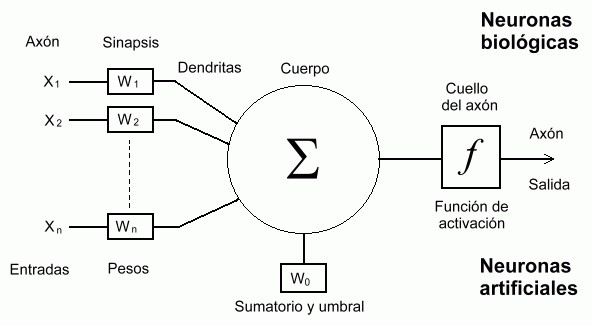
\includegraphics[width=0.9\textwidth]{neurona_artificial}
\caption[Diferenciación entre una neurona biológica y una neurona artificial]{Diferenciación entre una neurona biológica y una neurona artificial.
\newline
Imagen extraída de \url{http://www.cs.us.es/~fsancho/?e=72}}
\label{fig}
\end{figure}
\FloatBarrier

\subsection{Perceptrón}
 Un perceptrón es el modelo más simple de una neurona artificial, está basado en una única neurona y posee una única salida. El perceptrón puede combinarse con otros tipos de perceptrones o neuronas artificiales para formar una red neuronal mas compleja.
 
 A su vez, un perceptrón puede organizar sus neuronas en capas: capa de entrada, una capa de salida, y múltiples capas ocultas formadas por neuronas. En el caso de existir capas ocultas nos referimos a la red neuronal como perceptrón multicapa\footnote{\url{https://es.wikipedia.org/wiki/Perceptron\_multicapa}}.

\FloatBarrier
\begin{figure}[!h]
\centering
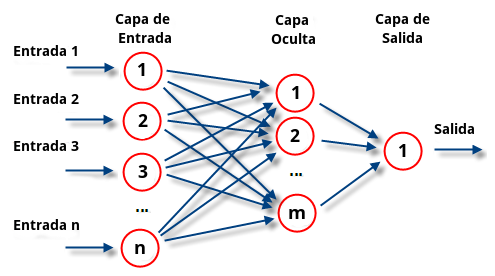
\includegraphics[width=0.9\textwidth]{perceptron_multicapa}
\caption[Diagrama de un  perceptrón multicapa]{Diagrama de un  perceptrón multicapa. Imagen extraída de
\newline
\url{https://es.wikipedia.org/wiki/Perceptron\_multicapa}}
\label{fig}
\end{figure}
\FloatBarrier

\section{Minería de datos}

La minería de datos se considera un campo de la estadística y de las ciencias de la computación. El proceso de la minería de datos se basa en el descubrimiento de patrones en grandes conjuntos de datos utilizando métodos de inteligencia artificial, aprendizaje automático, estadística y bases de datos. El principal objetivo es el de extraer información de un conjunto de datos y procesarlo para transformarlo de forma estructurada y comprensible para su uso posterior \cite{wiki:mineria_de_datos}.

El proceso típico de minería de datos está constituido por los siguientes pasos generales:

\begin{description}
    \item[Selección del \english{dataset} o conjunto de datos] Selección de los campos que se quieren predecir y de los necesarios para el proceso.
    \item[Análisis de las propiedades de los datos] Comprobación de histogramas, diagramas de dispersión y búsqueda de valores atípicos o nulos.
    \item[Transformación del conjunto de datos de entrada] Preparación de los datos obtenidos para aplicar la técnica de minería de datos que mejor se adapte al problema a resolver.
    \item[Selección y aplicación de la técnica de minería de datos] Construcción del modelo a aplicar: predictivo, o de clasificación.
    \item[Extracción de datos] Proceso por el que se recopilan los datos a ser tratados, ya sea registrando las medidas de sensores, consultando bases de datos, o como en este proyecto, realizando tareas de \english{web scraping}.
    \item[Interpretación y evaluación] Una vez obtenido el modelo, se procede a su validación y evaluación.
\end{description}

\subsection{Técnicas de minería de datos}
\begin{description}
    \item[Redes neuronales] Tal y como se han descrito anteriormente, esta técnica de procesamiento automático y los diferentes tipos de red neuronal (perceptrón y perceptrón multicapa) son una técnica utilizada en la minería de datos.
    \item[Regresión lineal] Técnica utilizada para identificar relaciones lineales entre dos variables.
    
    \FloatBarrier
    \begin{figure}[!h]
    \centering
    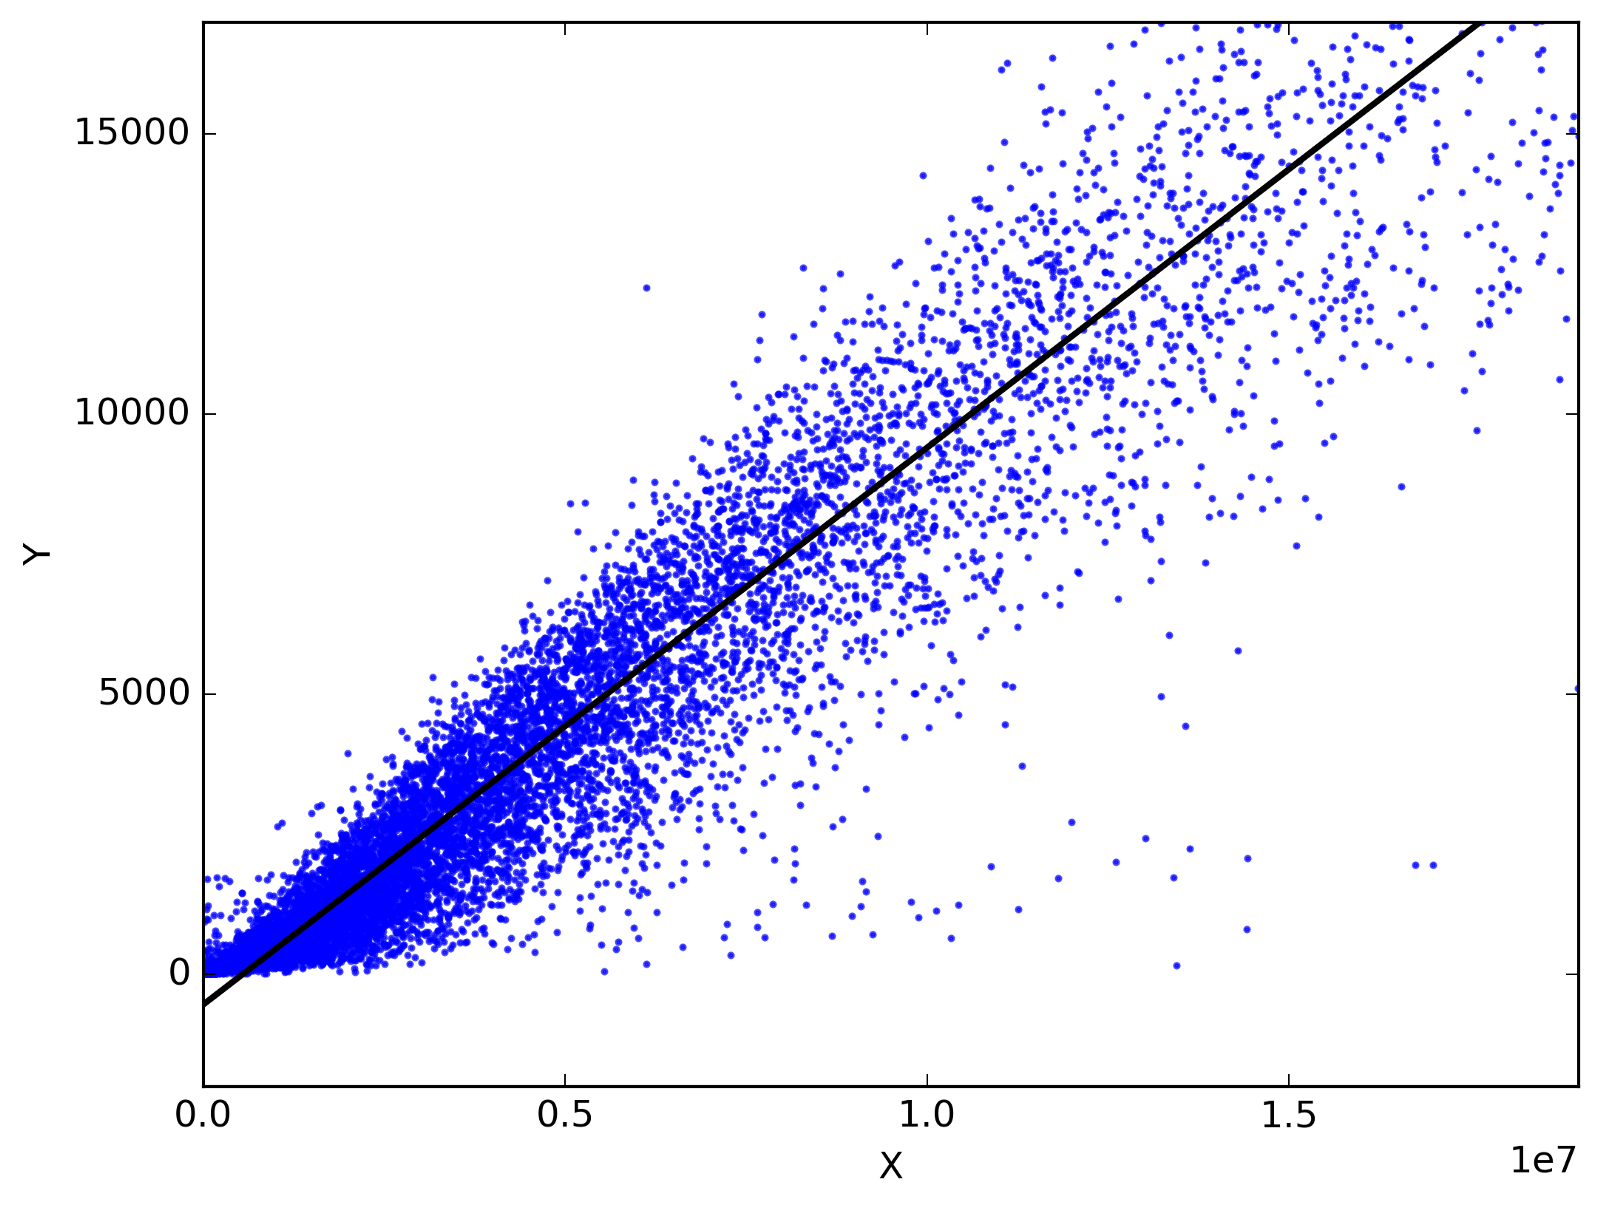
\includegraphics[width=0.7\textwidth]{regresion_lineal}
    \caption[Ejemplo de diagrama de regresión lineal]{Ejemplo de diagrama de regresión lineal.
    \newline
    Imagen extraída de \url{https://es.wikipedia.org/wiki/Regresion\_lineal}}
    \label{fig}
    \end{figure}
    \FloatBarrier
    
    \item[Árboles de decisión] Modelo de predicción utilizado en el campo de la inteligencia artificial y el análisis predictivo\footnote{\url{https://es.wikipedia.org/wiki/Analisis\_predictivo}} donde a partir de un conjunto de datos se construyen diagramas para representar y categorizar condiciones de forma sucesiva hasta resolver el problema dado.
    
    %\FloatBarrier
    %\begin{figure}[!h]
    %\centering
    %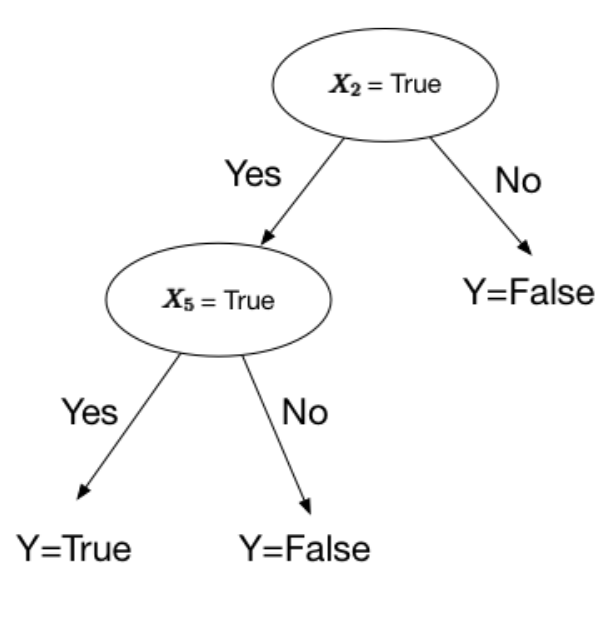
\includegraphics[width=0.5\textwidth]{arbol_decision}
    %\caption[Ejemplo de árbol de decisión]{Ejemplo de árbol de decisión.
    %\newline
    %Imagen extraída de
    %\newline
    %\url{https://hackernoon.com/what-is-a-decision-tree-in-machine-learning-15ce51dc445d}}
    %\label{fig}
    %\end{figure}
    %\FloatBarrier
    
    \item[Modelos estadísticos]Expresión o ecuación utilizada con el fin de indicar diferentes factores que modifican la variable de una respuesta.
    \item[Reglas de asociación] Procedimiento utilizado para reconocer hechos en común dentro de un conjunto de datos.
    \item[\english{Clustering}] Proceso de agrupación de una series de valores según un criterio de distancia o similitud.
    
    \FloatBarrier
    \begin{figure}[!h]
    \centering
    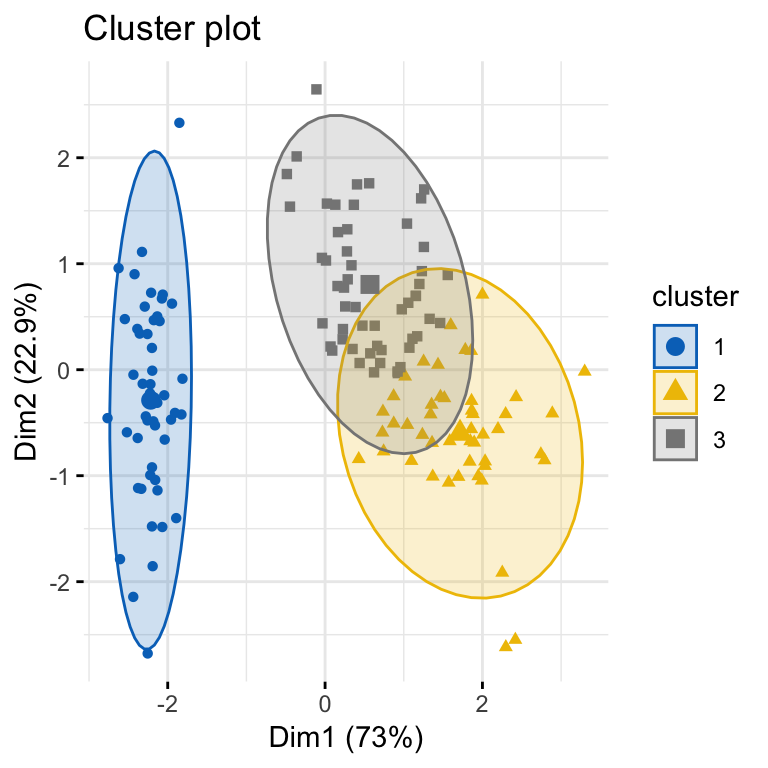
\includegraphics[width=0.7\textwidth]{clustering}
    \caption[Ejemplo de diagrama mostrando \english{clustering}]{Ejemplo de diagrama mostrando \english{clustering}.
    \newline
    Imagen extraída de \url{https://en.wikipedia.org/wiki/Cluster\_analysis}}
    \label{fig}
    \end{figure}
    \FloatBarrier
    
\end{description}

\section{Web Scraping}
El \english{web scraping} es un a técnica utilizada para extraer información desde páginas web a través de uno o varias herramientas de software, estos programas simulan la navegación por el sitio web a la hora de extraer los datos deseados. La técnica de web \english{scraping} es muy utilizada a día de hoy por servicios como motores de búsqueda ya que es necesario para indexar la web, sin embargo, los principales usos de esta técnica son la transformación de datos sin estructurar que podemos encontrar en cualquier web en formato HTML\footnote{\url{https://es.wikipedia.org/wiki/HTML}} a estructuras de datos que pueden ser almacenados en bases de datos, hojas de cálculo, o en cualquier forma de almacenamiento estructurada \cite{wiki:web_scraping}.

\newpage

En cuanto a las técnicas utilizadas para realizar \english{web scraping} sobre un sitio web encontramos varios tipos en función del nivel de automatización del proceso:

\begin{description}
    \item[Expresiones regulares] Es posible extraer información de una página web utilizando expresiones regulares.
    \item[Peticiones HTTP] Se basa en extraer información por medio de peticiones HTTP al servidor remoto utilizando sockets.
    \item[Algoritmos de minería de datos] Aplicación de algunas de las técnicas de minería de datos tratadas en el apartado anterior.
    \item[Parser HTML] Existen lenguajes capaces de procesar documentos HTML y extraer de forma estructurada todo el contenido de una web.
    \item[Aplicaciones de web scraping] Programas completos de \english{web scraping} que combinan algunas de las técnicas anteriores para ofrecer un proceso personalizado para cada caso, facilitando y simplificando la extracción del código de la aplicación de obtención de datos a partir de páginas web.
\end{description}